\documentclass[letterpaper,12pt,fleqn]{article}
\usepackage{matharticle}
\usepackage{tikz}
\pagestyle{plain}
\begin{document}

\begin{center}
  \large
  Math-19 Section 1

  \Large
  Homework \#1 Solutions
\end{center}

\subsection*{Problems}

\begin{enumerate}
\item We have stated in class that there may be multiple syntaxes to represent each point on the real number line.
  For example, we saw how to convert finite decimal and infinite repeating decimal forms to rational numbers in
  integer ratio form.
  \begin{enumerate}
  \item Convert the rational number \(0.\overline{1}\) to integer ratio form using the process that we learned in
    class.

    There are no fixed digits, and only one digit in the repeating pattern:
    \begin{gather*}
      x=0.\overline{1} \\
      10x=1.\overline{1} \\
      \\
      9x=1 \\
      x=\frac{1}{9}
    \end{gather*}
  \item Without repeating the process, fill in the following table:
    
    \renewcommand{\arraystretch}{2}
    \begin{tabular}{|c|p{0.25in}|}
      \hline
      \(0.\overline{1}\) & \(\frac{1}{9}\) \\
      \hline
      \(0.\overline{2}\) & \(\frac{2}{9}\) \\
      \hline
      \(0.\overline{3}\) & \(\frac{3}{9}\) \\
      \hline
      \(0.\overline{4}\) & \(\frac{4}{9}\) \\
      \hline
      \(0.\overline{5}\) & \(\frac{5}{9}\) \\
      \hline
      \(0.\overline{6}\) & \(\frac{6}{9}\) \\
      \hline
      \(0.\overline{7}\) & \(\frac{7}{9}\) \\
      \hline
      \(0.\overline{8}\) & \(\frac{8}{9}\) \\
      \hline
    \end{tabular}

  \item Based on this pattern, predict what \(0.\overline{9}\) equals.  Prove this by repeating the process to
    convert it to an integer ration.
    \begin{gather*}
      \frac{9}{9}=1
      \\
      x=0.\overline{9} \\
      10x=9.\overline{9} \\
      \\
      9x=9 \\
      x=1
    \end{gather*}
  \item Explain why the answer you got in the previous problem is valid.

    Because \(0.\overline{9}\) gets arbitrarily close to 1.

  \item Without repeating the process, what do you think \(25.3\overline{9}\) equals?
    \[25.4\]
  \end{enumerate}

\newcommand{\tick}[1]{\draw (#1,0.1) -- (#1,-0.1)}
\newcommand{\ocirc}[1]{\draw (#1,0) circle [radius=0.1]}
\newcommand{\ccirc}[1]{\draw [fill=black] (#1,0) circle [radius=0.1]}

\item Consider the following two sets:
  \begin{gather*}
    A=\setb{x\in\R}{-1<x\le3} \\
    B=\setb{x\in\R}{x>2}
  \end{gather*}
  Show the graph and the interval notation for each of the following:
  \begin{enumerate}
  \item \(A\)

    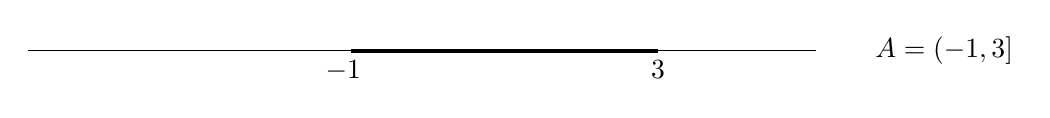
\begin{tikzpicture}
      \draw (-5,0) -- (5,0) node [right=0.25in] {\(A=(-1,3]\)};
      \tick{-1};
      \tick{3};
      \ocirc{-1};
      \ccirc{3};
      \draw [ultra thick] (-0.9,0) -- (3,0);
      \node [below] at (-1,0) {\(-1\)};
      \node [below] at (3,0) {\(3\)};
    \end{tikzpicture}
  
  \item \(B\)

    \begin{tikzpicture}
      \draw (-5,0) -- (5,0) node [right=0.25in] {\(B=(2,\infty)\)};
      \tick{2};
      \ocirc{2};
      \draw [->, ultra thick] (2.1,0) -- (5,0);
      \node [below] at (2,0) {\(2\)};
    \end{tikzpicture}

  \item \(A\cap B\)

    \begin{tikzpicture}
      \draw (-5,0) -- (5,0) node [right=0.25in] {\(A\cap B=(2,3]\)};
      \tick{2};
      \tick{3};
      \ocirc{2};
      \ccirc{3};
      \draw [ultra thick] (2.1,0) -- (3,0);
      \node [below] at (2,0) {\(2\)};
      \node [below] at (2,0) {\(2\)};
    \end{tikzpicture}

  \item \(A\cup B\)

    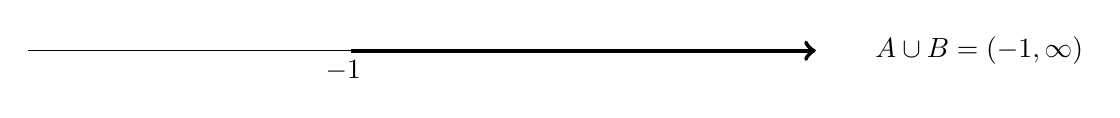
\begin{tikzpicture}
      \draw (-5,0) -- (5,0) node [right=0.25in] {\(A\cup B=(-1,\infty)\)};
      \tick{-1};
      \ocirc{-1};
      \draw [->,ultra thick] (-0.9,0) -- (5,0);
      \node [below] at (-1,0) {\(-1\)};
    \end{tikzpicture}

  \item \(A-B\)

    \begin{tikzpicture}
      \draw (-5,0) -- (5,0) node [right=0.25in] {\(A-B=(-1,2]\)};
      \tick{-1};
      \tick{2};
      \ocirc{-1};
      \ccirc{2};
      \draw [ultra thick] (-0.9,0) -- (2,0);
      \node [below] at (-1,0) {\(-1\)};
      \node [below] at (2,0) {\(2\)};
    \end{tikzpicture}
  \end{enumerate}


\item Simplify the following expression. Your answer should contain no radicals and no negative exponents. You may
  assume that $a,b,c>0$.  Hint: convert all the ugly radicals to rational exponents and be care with parentheses: note
  that there is a radical within a radical.
  \[\frac{a^2b^{-3}\sqrt{abc^3}}{\sqrt[3]{a^{-2}\sqrt{b^3c}}}\]
  \begin{align*}
    \frac{a^2b^{-3}\sqrt{abc^3}}{\sqrt[3]{a^{-2}\sqrt{b^3c}}} &=
    \frac{a^2b^{-3}(abc^3)^{\frac{1}{2}}}{(a^{-2}(b^3c)^{\frac{1}{2}})^{\frac{1}{3}}} \\
    &= \frac{a^2b^{-3}a^{\frac{1}{2}}b^{\frac{1}{2}}c^{\frac{3}{2}}}{(a^{-2}b^{\frac{3}{2}}c^{\frac{1}{2}})^{\frac{1}{3}}} \\
    &= \frac{a^{\frac{5}{2}}b^{\frac{-5}{2}}c^{\frac{3}{2}}}{a^{-\frac{2}{3}}b^{\frac{1}{2}}c^{\frac{1}{6}}} \\
    &= a^{\frac{19}{6}}b^{-3}c^{\frac{8}{6}} \\
    &= \frac{a^{\frac{19}{6}}c^{\frac{4}{3}}}{b^3}
  \end{align*}

\item Determine whether each of the following statements is either correct, incorrect, or misleading.  Explain why
  incorrect and misleading statements are incorrect or misleading are fix them so that they are correct.
  \begin{enumerate}
  \item \(\sqrt{9}=\pm3\)

    This statement is incorrect.  \(\sqrt{9}\) asks for the positive value.  If we specifically want the negative
    value, then we need to preceed the radical by a negative sign:
    \begin{gather*}
      \sqrt{9}=3 \\
      -\sqrt{9}=-3
    \end{gather*}
  \item \(\left(x^{\frac{1}{2}}\right)^2=\abs{x}\)

    This statement is misleading.  \(x^{\frac{1}{2}}\) implies that \(x\ge0\), so the absolute value is not needed:
    \[\left(x^{\frac{1}{2}}\right)^2=x\]
  \item \(\left(x^2\right)^{\frac{1}{2}}=x\)
    This statement is incorrect: absolute value is needed here:
    \[\left(x^2\right)^{\frac{1}{2}}=\abs{x}\]
  \item \(\left(x^3\right)^{\frac{1}{3}}=\abs{x}\)
    This statement is incorrect: absolute value is not needed for odd roots:
    \[\left(x^3\right)^{\frac{1}{3}}=x\]
  \end{enumerate}

\end{enumerate}

\end{document}
